\documentclass{ctexart}

\usepackage{graphicx}
\usepackage{subcaption}
\usepackage{float}

\title{实验一报告}
\author{唐宇恩 \quad 251220100}
\date{\today}

\begin{document}
\maketitle

\section{3输入多数表决器}

\subsection{整体方案设计}
这就只有一个模块，共三个输入 $X,Y,Z$ ，一个输出 $F$ ，满足

\[
F = XY + YZ + ZX
\]

\subsection{实验电路图}

\begin{figure}[htbp]
    \centering
    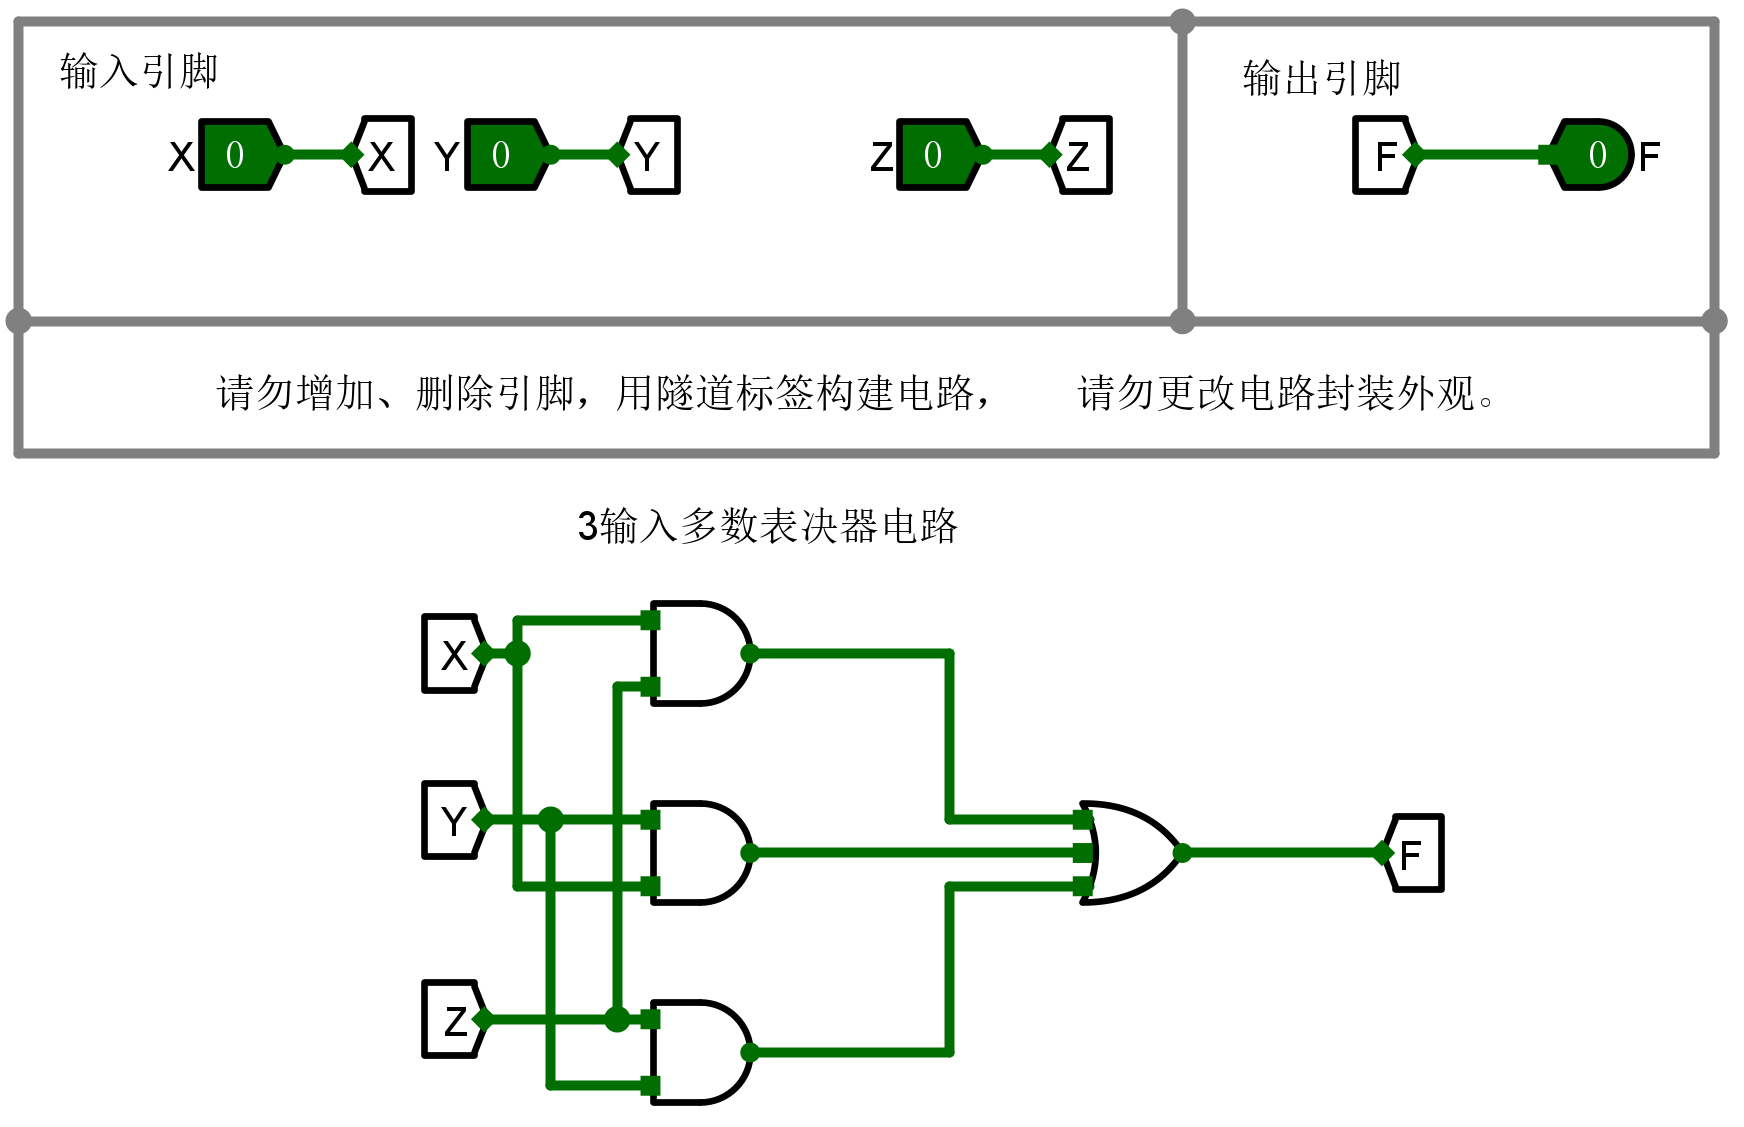
\includegraphics[width=0.8\textwidth]{assets/lab1-1.png}
    \caption{电路图}
\end{figure}

\subsection{真值表验证}

\begin{tabular}{ccc|c}
$X$ & $Y$ & $Z$ & $F$ \\
\hline
0 & 0 & 0 & 0 \\
0 & 0 & 1 & 0 \\
0 & 1 & 0 & 0 \\
0 & 1 & 1 & 1 \\    
1 & 0 & 0 & 0 \\
1 & 0 & 1 & 1 \\
1 & 1 & 0 & 1 \\
1 & 1 & 1 & 1 \\
\end{tabular}

\section{CMOS两输入或门}

\subsection{整体方案设计}

使用CMOS或非门和CMOS非门串行以实现CMOS或门.

\subsection{实验电路图}

\begin{figure}[htbp]
    \centering
    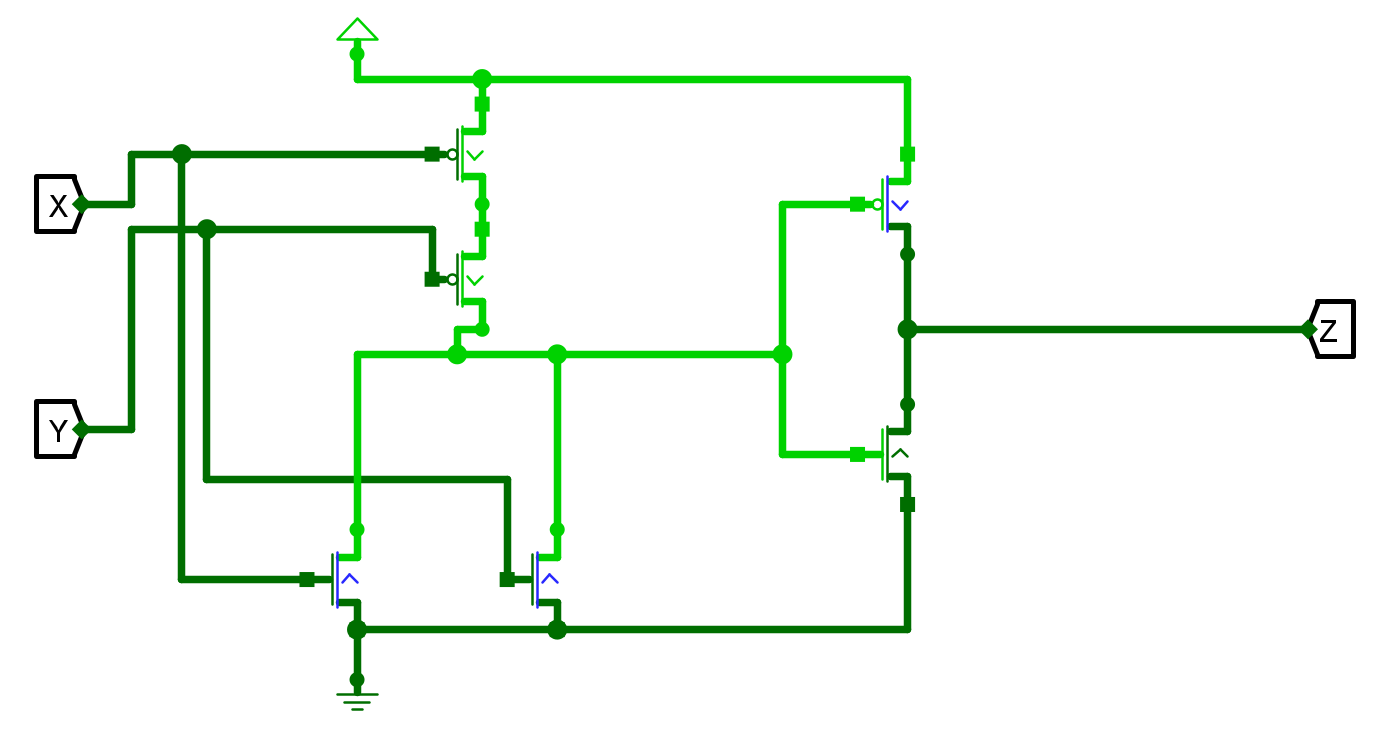
\includegraphics[width=0.8\textwidth]{assets/lab1-2.png}
    \caption{电路图}
\end{figure}

\subsection{真值表验证}

\begin{tabular}{cc|c}
$X$ & $Y$ & $Z$ \\
\hline
0 & 0 & 0 \\
0 & 1 & 1 \\
1 & 0 & 1 \\
1 & 1 & 1 \\
\end{tabular}

\section{利用基本逻辑门和CMOS实现多路选择器}

\subsection{整体方案设计}

共三个输入，$D_0, D_1$ 和一个选择信号 $S$，输出为 $Y$.

\[
Y = \overline{S}D_0 + SD_1
\]

\subsection{实验电路图}

\begin{figure}[htbp]
    \centering
    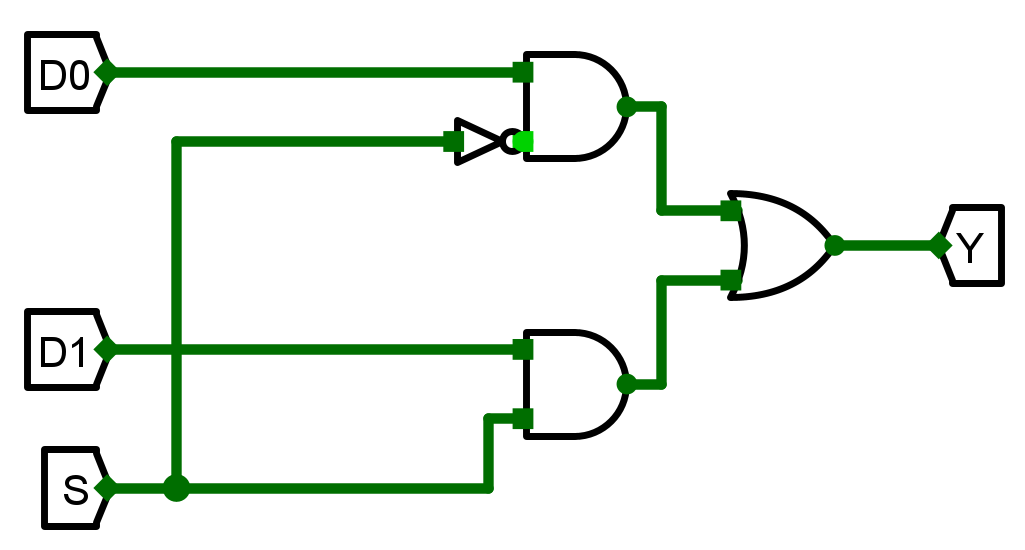
\includegraphics[width=0.8\textwidth]{assets/lab1-3.png}
    \caption{电路图}
\end{figure}

\subsection{真值表验证}

\begin{tabular}{ccc|c}
$D0$ & $D1$ & $S$ & $Y$ \\
\hline
0 & 0 & 0 & 0 \\
0 & 0 & 1 & 0 \\
0 & 1 & 0 & 0 \\
0 & 1 & 1 & 1 \\
1 & 0 & 0 & 1 \\
1 & 0 & 1 & 0 \\
1 & 1 & 0 & 1 \\
1 & 1 & 1 & 1 \\
\end{tabular}

\section{利用晶体管和传输门实现多路选择器}

\subsection{整体方案设计}

本二选一多路选择器采用 $D0, D1$ 作为输入，$S$ 作为选择信号. 输出为 $Y$.

\subsection{实验电路图}

\begin{figure}[htbp]
    \centering
    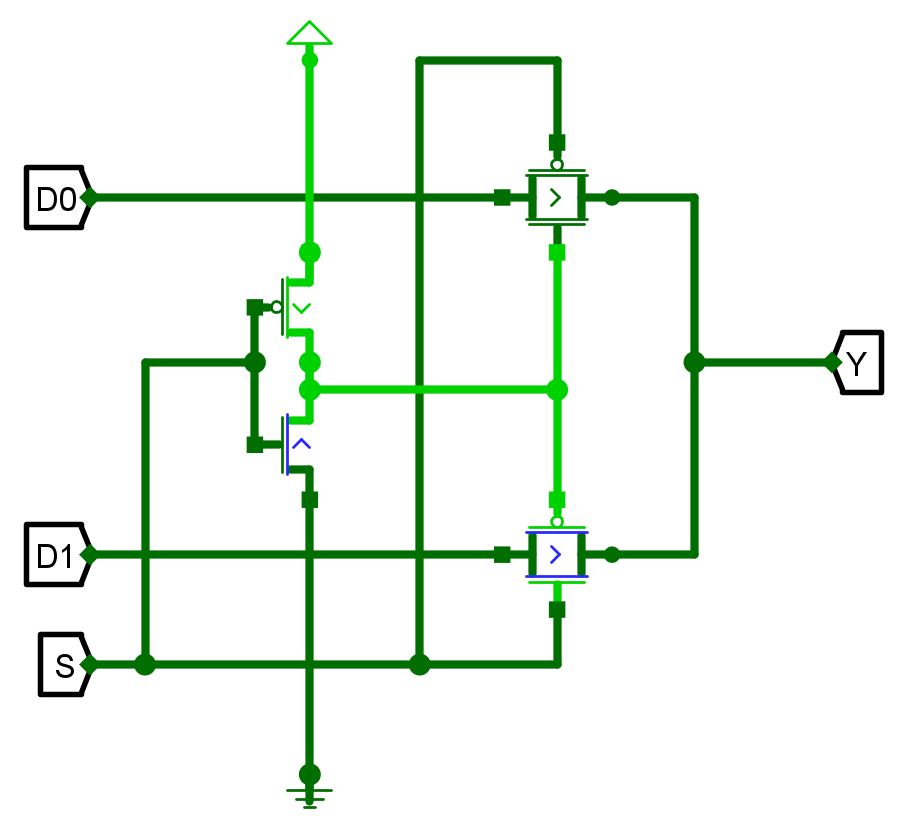
\includegraphics[width=0.8\textwidth]{assets/lab1-4.png}
    \caption{电路图}
\end{figure}

\subsection{真值表验证}

\begin{tabular}{ccc|c}
$D0$ & $D1$ & $S$ & $Y$ \\
\hline
0 & 0 & 0 & 0 \\
0 & 0 & 1 & 0 \\
0 & 1 & 0 & 0 \\
0 & 1 & 1 & 1 \\
1 & 0 & 0 & 1 \\
1 & 0 & 1 & 0 \\
1 & 1 & 0 & 1 \\
1 & 1 & 1 & 1 \\
\end{tabular}

\section{子电路级联实验}

\subsection{整体方案设计}

使用3个二路选择器级联实现一个4路选择器. 输入为 $D0, D1, D2, D3$ 和选择信号 $S0, S1$，输出为 $Y$.
先实现一个二路选择器作为子模块，输入为 $D0, D1$ 和选择信号 $S0$，输出为 $Y0$.
然后利用二路选择器实现这个四路选择器.

\subsection{实验电路图}

\begin{figure}[htbp]
    \centering
    \begin{subfigure}{0.4\textwidth}
        \centering
        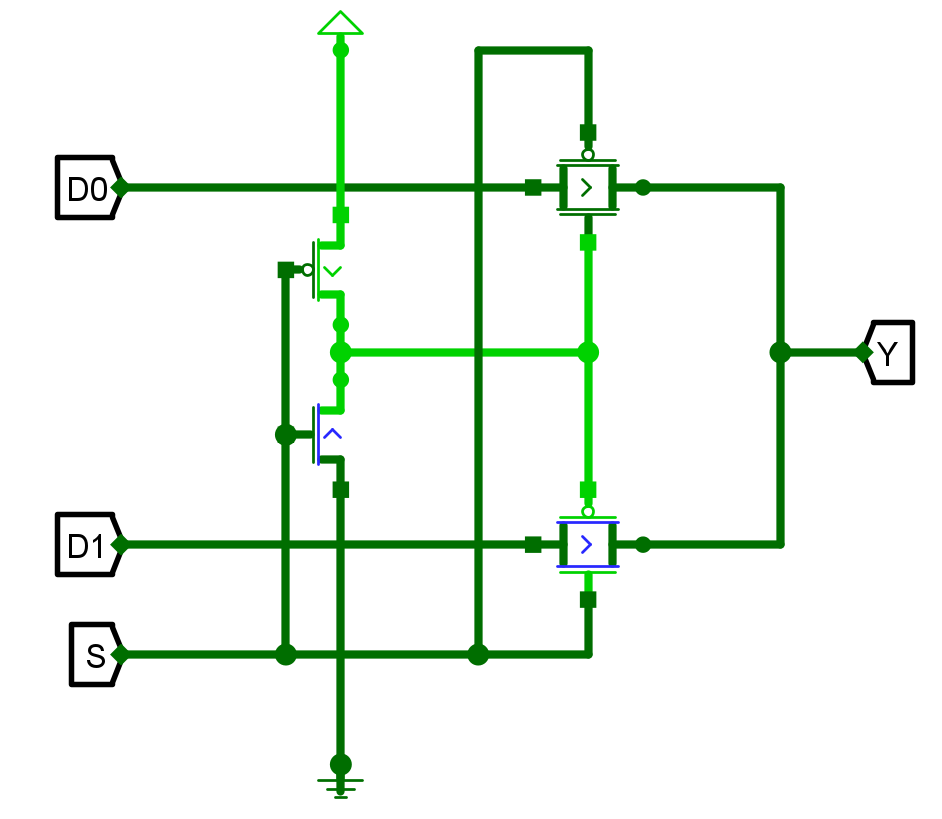
\includegraphics[width=0.8\textwidth]{assets/lab1-5-1.png}
        \caption{二路选择器子模块电路图}
    \end{subfigure}
    \begin{subfigure}{0.4\textwidth}
        \centering
        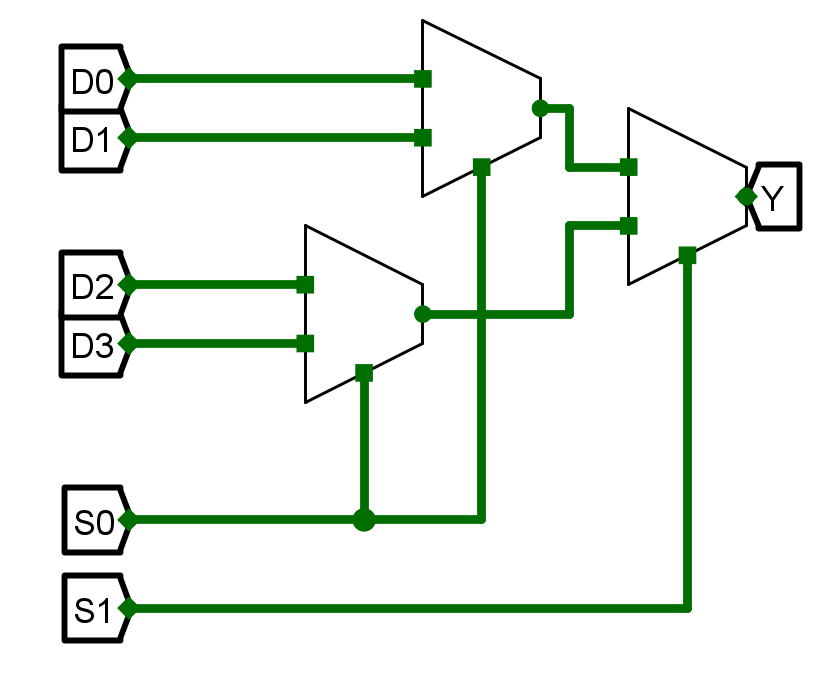
\includegraphics[width=0.8\textwidth]{assets/lab1-5-2.png}
        \caption{四路选择器电路图}
    \end{subfigure}
    \caption{电路图}
\end{figure}

\section{思考题}

\subsection{根据 2 选 1 多路选择器的与-或电路，替换成与非-与非电路，并分析两种电路的特性}

二选一多路选择器的与非-与非电路如下图所示：

\begin{figure}[H]
    \centering
    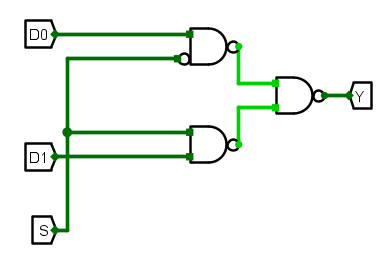
\includegraphics[width=0.8\textwidth]{assets/lab1-ec1.png}
    \caption{与非-与非电路}
\end{figure}

采用与非-与非门可以减少使用的晶体管数量，降低延迟和功耗.
与-或电路和与非-与非电路框架相似，但是逻辑上更加简洁.

\subsection{实现 4 位二进制数转换成格雷码的转换电路}

格雷码是一种特殊的二进制编码方式，具有相邻码之间只有一位不同的特点.以二进制为0值的格雷码为第零项，第一项改变最右边的位元，第二项改变右起第一个为1的位元的左边位元，第三、四项方法同第一、二项，如此反复，即可排列出n个位元的格雷码。可以知道，第 $n$ 位格雷码等于第 $n$ 位二进制数异或第 $n$ 位二进制数右移一位的结果，即

\[
G_n = I_n \oplus (I_n >> 1) = I_n \oplus I_{n+1}
\]

采用 $I0,I1,I2,I3$ 表示4位二进制数，$G0,G1,G2,G3$ 表示对应的格雷码.
4位二进制数转换成格雷码的转换电路如下图所示：

\begin{figure}[H]
    \centering
    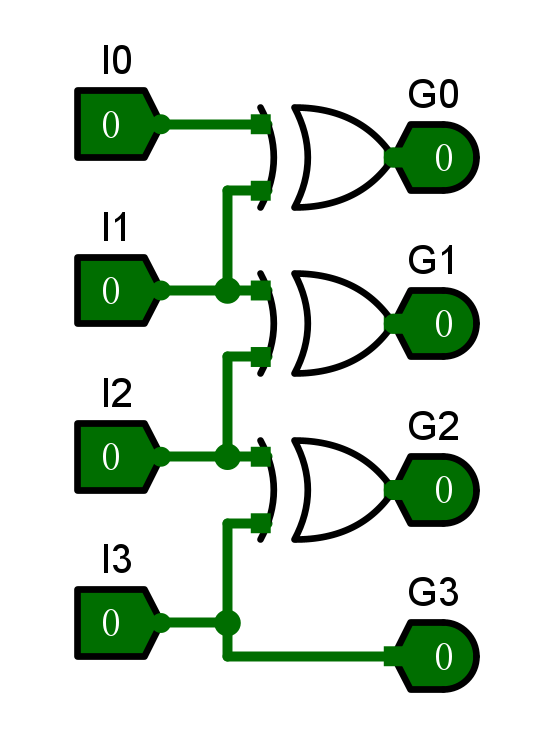
\includegraphics[width=0.6\textwidth]{assets/lab1-ec2.png}
    \caption{4位二进制数转换成格雷码的转换电路}
\end{figure}

\subsection{实现 4 位二进制数的奇偶校验位生成电路}

奇偶校验位是指使得加入校验位后，整个二进制数中1的个数为偶数（偶校验）或奇数（奇校验）.4位二进制数 $I0,I1,I2,I3$ 的偶校验位 $P_{even}$ 和奇校验位 $P_{odd}$ 可以通过以下公式计算：

\[
P_{even} = I0 \oplus I1 \oplus I2 \oplus I3
\]
\[
P_{odd} = \overline{P_{even}}
\]

4位二进制数的奇偶校验位生成电路如下图所示：

\begin{figure}[H]
    \centering
    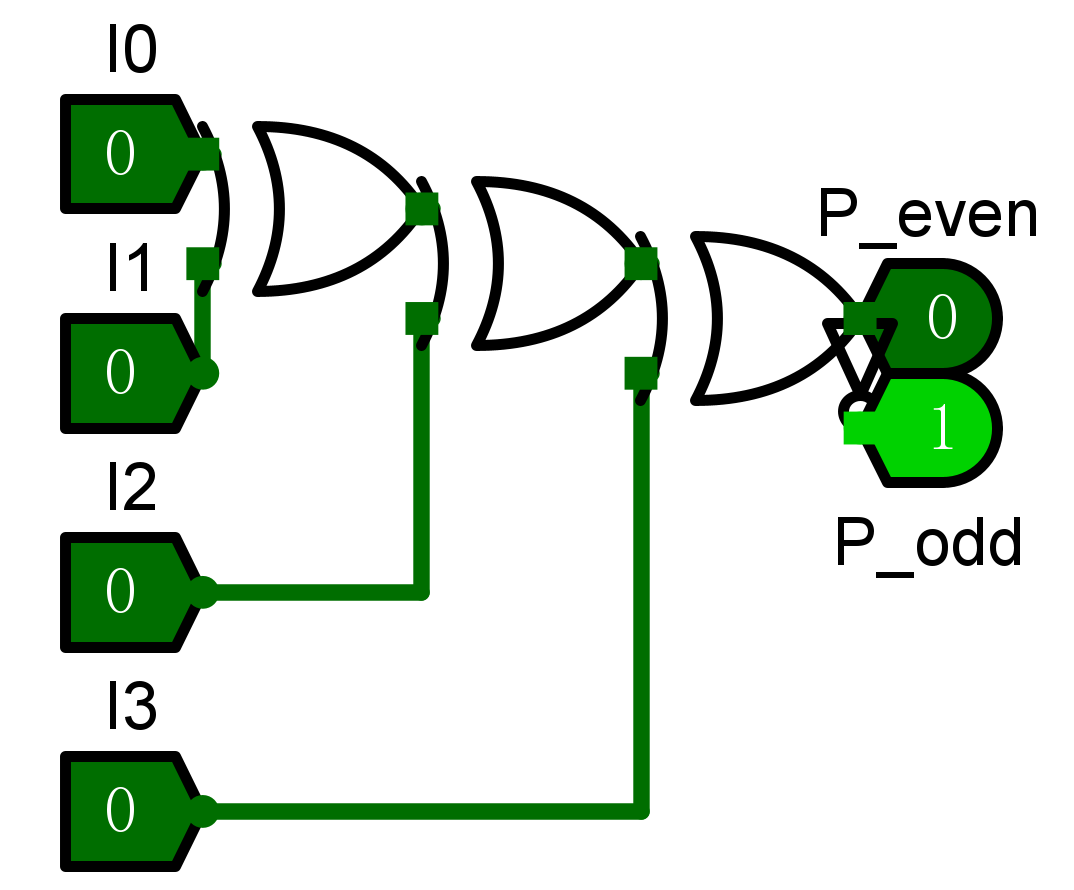
\includegraphics[width=0.6\textwidth]{assets/lab1-ec3.png}
    \caption{4位二进制数的奇偶校验位生成电路}
\end{figure}

\end{document}